\documentclass[10pt,a4paper]{article}
\usepackage[T1]{fontenc}
\usepackage[utf8]{inputenc}
\usepackage{lmodern}
\usepackage[a4paper,margin=2.5cm]{geometry}
\usepackage{setspace}
\usepackage{microtype}
\usepackage{booktabs,tabularx,array}
\usepackage{tikz}
\usepackage{float}
\usepackage{hyperref}
\usepackage{enumitem}

\hypersetup{colorlinks=true,urlcolor=blue,linkcolor=black}

\setlength{\parindent}{0pt}
\setlength{\parskip}{2pt}
\setlength{\textfloatsep}{5pt}
\setlength{\intextsep}{5pt}
\setlength{\abovecaptionskip}{3pt}
\setlength{\belowcaptionskip}{2pt}

\setlist{nosep,leftmargin=1.4em}
\renewcommand{\arraystretch}{1.12}

\onehalfspacing
\raggedbottom

\title{Laporan Preprocessing dan Integrasi Data Kecelakaan Lalu Lintas Chicago, Periode 2018--2025}
\author{Ahmad Maulana Ibrahim\\24/539655/TK/59853}
\date{}

\begin{document}
\maketitle
\vspace{-1.2em}

\section{Pemeriksaan Data dan Seleksi Atribut Awal}

Data berasal dari tiga tabel terbuka City of Chicago: \emph{Traffic Crashes--Crashes},
\emph{Traffic Crashes--Vehicles}, dan \emph{Traffic Crashes--People}. Crashes
memuat satu baris untuk setiap kecelakaan, Vehicle satu baris untuk setiap unit
yang terlibat, dan People satu baris untuk setiap orang. Ketiganya dapat
dihubungkan dengan \texttt{crash\_record\_id}. Berkas yang dianalisis mencakup
tahun 2018--2025.\footnote{Sumber: \url{https://data.cityofchicago.org/d/85ca-t3if},
\url{https://data.cityofchicago.org/d/68nd-jvt3}, dan
\url{https://data.cityofchicago.org/d/u6pd-qa9d}.}

\begin{table}[H]
\centering\small
\caption{Kondisi awal ketiga tabel. Persentase kosong dihitung dari semua sel pada masing-masing tabel.}
\begin{tabular}{lrrrr}
\toprule
Tabel & Baris & Kolom & Sel kosong & Kosong (\%)\\
\midrule
Crashes & 877.921 & 49 & 9.001.923 & 20,93\\
Vehicle & 1.792.372 & 71 & 93.017.957 & 73,09\\
People & 1.927.657 & 29 & 22.063.385 & 39,47\\
\bottomrule
\end{tabular}
\end{table}

Dataset dipilih karena memuat waktu, lokasi, kondisi jalan, jenis kendaraan,
dan cedera orang. Ketiga sumber dapat menjawab pertanyaan lokasi, waktu, dan
keterlibatan kendaraan, tetapi tingkat kekosongannya berbeda. Pemeriksaan
awal menghitung baris, kolom, sel kosong, serta duplikat; tidak ditemukan
baris atau ID ganda.

Sebelum cleaning, notebook mengeluarkan atribut yang kosong pada lebih dari
30\% baris tabelnya. Aturan ini hanya berlaku untuk kolom; seluruh
4.597.950 baris dipertahankan. Kolom yang jarang terisi tidak dipakai dalam
analisis umum agar tidak memerlukan terlalu banyak tebakan.

\begin{table}[H]
\centering\small
\caption{Seleksi atribut awal berdasarkan batas lebih dari 30\% nilai kosong.}
\begin{tabular}{lrrr}
\toprule
Sumber & Kolom awal & Dikeluarkan & Kolom tersisa\\
\midrule
Crashes & 49 & 11 & 38\\
Vehicle & 71 & 54 & 17\\
People & 29 & 12 & 17\\
\midrule
Total & 149 & 77 & 72\\
\bottomrule
\end{tabular}
\end{table}

Contoh atribut yang dikeluarkan adalah \texttt{work\_zone\_type} pada
Crashes, atribut trailer pada Vehicle, dan \texttt{hospital} pada People.
CSV mentah tetap disimpan untuk kajian yang membutuhkan atribut tersebut.

\section{Data Cleaning: Apa yang Diperbaiki dan Mengapa}

Cleaning dilakukan tanpa menghapus baris sumber. Setiap perubahan dicatat
agar nilai asli, nilai yang diperbaiki, dan nilai yang masih belum diketahui
dapat dibedakan.

\begin{enumerate}
\item \textbf{Tulisan kosong dan format.} Spasi di awal/akhir dibuang; sel yang
hanya berisi spasi diseragamkan menjadi kosong. Tanggal dan angka dibaca
sesuai jenisnya. Langkah ini tidak mengisi nilai (0 sel); jumlah spasi yang
dirapikan tidak dicatat terpisah dalam audit.
\item \textbf{Nilai tidak masuk akal.} Sebanyak 8 nilai \texttt{age} di luar
0--120 tahun dan 1.073 nilai \texttt{vehicle\_year} yang tidak wajar
dijadikan kosong: total 1.081 nilai ditandai, bukan diisi. Nilai asal
disimpan pada \texttt{age\_raw} dan \texttt{vehicle\_year\_raw}.
\item \textbf{Kategori yang kosong.} Pada kolom sumber, 3.314.281 sel diberi
label status, bukan nilai faktual: 33.915 sel Crashes, 567.402 sel Vehicle,
dan 2.712.964 sel People. Label \texttt{TIDAK\_BERLAKU} digunakan ketika
atribut tidak berlaku; \texttt{TIDAK\_TERCATAT} ketika informasinya tidak ada.
Contohnya, \texttt{report\_type} diisi status 31.920 kali; enam atribut
unit nonkendaraan, termasuk \texttt{make} dan \texttt{model}, masing-masing
41.431 kali diberi status tidak berlaku. Jumlah ini adalah sel, bukan baris unik.
\item \textbf{Pemeriksaan silang kolom sumber.} Kode memeriksa apakah
koordinat dapat diperoleh dari teks \texttt{location} dan apakah total
cedera dapat dijumlahkan dari empat komponen yang lengkap. Pada data ini
kedua cara tersebut tidak menambah pengisian (0 sel). Nilai tanpa bukti
yang cukup tetap kosong atau diberi label tidak tercatat.
\end{enumerate}

Audit cleaning membedakan nilai sumber, label kategori, dan perkiraan.
Tidak ada ID atau baris ganda yang dibuang. Perbandingan jumlah sel kosong
disajikan setelah seluruh tahap pada Bagian 6.

\section{Transformasi, Estimasi, dan Pemetaan Lokasi}

Transformation mengubah bentuk atau menambah kolom agar data dapat dihitung
dan dibandingkan. Kolom asli tetap tersedia jika sebuah perubahan bersifat
perkiraan.

\begin{table}[H]
\centering\footnotesize
\caption{Format awal kolom dan bentuk yang dipakai untuk analisis. Semua kolom CSV mula-mula dibaca sebagai teks.}
\begin{tabularx}{\linewidth}{p{3.3cm}
>{\raggedright\arraybackslash}X
>{\raggedright\arraybackslash}X}
\toprule
Kolom asal dan format awal & Hasil dan format baru & Alasan\\
\midrule
\texttt{crash\_date}: teks tanggal ISO & Tanggal dan jam (\texttt{datetime}); kolom bulan, hari, dan jam sumber dibaca sebagai bilangan bulat. & Mengurutkan kejadian menurut waktu.\\
\texttt{age}: teks angka atau kosong & Usia bilangan bulat; \texttt{age\_group} berupa kategori teks. & Membandingkan kelompok umur.\\
\texttt{age}, \texttt{vehicle\_year}: teks angka atau kosong & Salinan \texttt{age\_imputed} dan \texttt{vehicle\_year\_imputed} berupa angka; nilai kosong tertentu diisi median. & Memungkinkan analisis angka tanpa mengubah kolom asal.\\
\texttt{injuries\_total}: teks angka; \texttt{most\_severe\_injury}: kategori teks & Kolom perkiraan total cedera berupa bilangan bulat dan tingkat keparahan berupa teks. & Melengkapi kasus yang jelas tercatat ``tanpa cedera''.\\
\texttt{latitude}, \texttt{longitude}: teks angka desimal; \texttt{location}: teks WKT & Koordinat berupa angka desimal; nomor area berupa bilangan bulat dan nama area berupa teks. & Mengelompokkan titik kecelakaan menurut wilayah.\\
\bottomrule
\end{tabularx}
\end{table}

\begin{table}[H]
\centering\footnotesize
\caption{Contoh nilai sebelum dan sesudah transformasi dari hasil pemrosesan. Tanda ``kosong'' berarti nilai sumber tidak tersedia.}
\begin{tabularx}{\linewidth}{p{2.6cm}
>{\raggedright\arraybackslash}X
>{\raggedright\arraybackslash}X}
\toprule
Kolom & Sebelum (CSV) & Sesudah (kolom analisis)\\
\midrule
\texttt{crash\_date} & \texttt{2018-01-01T00:00:00.000} & \texttt{2018-01-01 00:00:00} (tanggal--jam)\\
\texttt{age} & \texttt{39} (teks) & 39 (angka); \texttt{age\_group = 25-44}\\
\texttt{age} kosong & Pengemudi perempuan; usia kosong & \texttt{age\_imputed = 36} (median kelompok)\\
\texttt{vehicle\_year} kosong & Nissan Altima; tahun kosong & \texttt{vehicle\_year\_imputed = 2013}\\
Kolom cedera kosong & \texttt{crash\_type}: tanpa cedera & \texttt{injuries\_total\_estimated = 0}; tingkat keparahan: tanpa cedera\\
Koordinat kosong & \texttt{latitude}, \texttt{longitude}: kosong & Estimasi 41,84613; $-87,69518$; area South Lawndale\\
\bottomrule
\end{tabularx}
\end{table}

Usia yang kosong pada salinan analisis diisi dengan median (nilai tengah) orang yang
mempunyai peran dan jenis kelamin sama; jika kelompoknya tidak cukup,
median peran saja dipakai. Sebanyak 556.320 nilai pada
\texttt{age\_imputed} terisi. Salinan tahun kendaraan diisi dengan median
merek--model yang memiliki sedikitnya 30 tahun kendaraan tercatat;
102.934 nilai terisi. Usia dan tahun kendaraan pada kolom asal tetap kosong
ketika nilainya tidak diketahui.

Sesudah cleaning, 1.159 dari 7.068 kecelakaan tanpa koordinat mendapat
perkiraan titik dari pencocokan alamat Census.\footnote{
\url{https://geocoding.geo.census.gov/geocoder/Geocoding_Services_API.html}.}
Pada 1.096 dari 1.987 kecelakaan tanpa \texttt{injuries\_total}, total
cedera diperkirakan nol dan tingkat keparahan diperkirakan ``tanpa cedera''
karena \texttt{crash\_type} menyatakan tidak ada cedera. Perkiraan berada
di kolom baru dengan penanda, sehingga nilai sumber tidak tertimpa.
Sebanyak 5.909 lokasi, 891 total cedera, dan 898 tingkat keparahan
masih belum diketahui.
Titik dengan koordinat yang dapat dipakai kemudian dicocokkan dengan batas
77 \emph{community area}\footnote{Batas wilayah:
\url{https://data.cityofchicago.org/d/igwz-8jzy}.}:
870.436 kecelakaan dari koordinat asli dan 1.150
dari koordinat estimasi masuk ke suatu area. Sebanyak 6.335 kecelakaan
tetap memiliki status area belum diketahui; tidak dipaksa masuk ke area
terdekat.

\section{Integrasi: Tiga Sumber Menjadi Enam Tabel}

Crashes dihubungkan dengan Vehicle dan People melalui
\texttt{crash\_record\_id}. Untuk menghubungkan satu orang ke satu unit,
digunakan \texttt{vehicle\_id} bersama ID kecelakaan yang sama. Pola
\texttt{person\_id} dipakai hanya jika hubungannya unik dan dapat diperiksa.
Jumlah orang dan kendaraan dihitung terlebih dahulu per kecelakaan, baru
ditambahkan ke Crashes. Dengan cara ini, dua orang dalam dua kendaraan
tidak berubah menjadi empat kecelakaan.

\begin{table}[H]
\centering\footnotesize
\caption{Enam tabel hasil integrasi dan ringkasan. ``Satu baris'' menentukan apa yang boleh dihitung.}
\begin{tabularx}{\linewidth}{p{4.5cm}rr>{\raggedright\arraybackslash}X}
\toprule
Tabel dan arti satu baris & Baris & Kolom & Isi utama\\
\midrule
\texttt{integrated\_crashes}: satu kecelakaan & 877.921 & 67 & Tanggal, kondisi, cedera, jumlah orang dan kendaraan, area, asal koordinat.\\
\texttt{integrated\_vehicles}: satu unit & 1.792.372 & 38 & Jenis, merek, model, kondisi kecelakaan, dan orang dalam unit yang terhubung.\\
\texttt{integrated\_people}: satu orang & 1.927.657 & 45 & Usia, cedera, lokasi, kondisi kecelakaan, dan konteks kendaraan jika tautannya pasti.\\
\texttt{area\_impact\_summary}: satu area & 77 & 13 & Kecelakaan, orang, korban, kendaraan, dan kejadian berat per area.\\
\texttt{hourly\_risk\_summary}: hari--jam & 168 & 9 & Kecelakaan, korban, kendaraan, dan kejadian berat untuk 7 hari $\times$ 24 jam.\\
\texttt{vehicle\_severity\_summary}: jenis--keparahan & 122 & 7 & Unit, kecelakaan unik yang melibatkan jenis itu, dan cedera penghuninya.\\
\bottomrule
\end{tabularx}
\end{table}

\begin{table}[H]
\centering\scriptsize
\caption{Lima community area dengan kecelakaan terbanyak dari \texttt{area\_impact\_summary}; kolom utama.}
\begin{tabular}{lrrrr}
\toprule
Area & Kecelakaan & Korban & Kendaraan & Kec. berat\\
\midrule
Austin & 41.495 & 10.695 & 84.238 & 868\\
Near West Side & 40.539 & 8.005 & 79.359 & 692\\
Near North Side & 38.912 & 6.333 & 74.604 & 549\\
Loop & 28.342 & 5.218 & 54.849 & 487\\
West Town & 25.581 & 5.096 & 50.309 & 457\\
\bottomrule
\end{tabular}
\end{table}

\begin{table}[H]
\centering\scriptsize
\caption{Lima kombinasi hari--jam dengan kecelakaan terbanyak dari \texttt{hourly\_risk\_summary}; kode hari mengikuti sumber.}
\begin{tabular}{rrrrr}
\toprule
Hari & Jam & Kecelakaan & Korban & Kec. berat\\
\midrule
6 & 15 & 11.630 & 2.144 & 147\\
6 & 16 & 11.437 & 2.153 & 169\\
6 & 17 & 10.902 & 1.953 & 160\\
5 & 16 & 10.560 & 2.037 & 144\\
5 & 15 & 10.494 & 2.040 & 130\\
\bottomrule
\end{tabular}
\end{table}

\begin{table}[H]
\centering\scriptsize
\caption{Lima kombinasi jenis kendaraan--keparahan dengan unit terbanyak dari \texttt{vehicle\_severity\_summary}; kolom utama.}
\begin{tabularx}{\linewidth}{>{\raggedright\arraybackslash}X
>{\raggedright\arraybackslash}Xrr}
\toprule
Jenis kendaraan & Keparahan kecelakaan & Unit & Kecelakaan unik\\
\midrule
PASSENGER & NO INDICATION OF INJURY & 918.720 & 604.539\\
SPORT UTILITY VEHICLE (SUV) & NO INDICATION OF INJURY & 217.685 & 181.301\\
UNKNOWN/NA & NO INDICATION OF INJURY & 142.211 & 132.796\\
PASSENGER & NONINCAPACITATING INJURY & 93.398 & 59.576\\
VAN/MINI-VAN & NO INDICATION OF INJURY & 66.617 & 63.805\\
\bottomrule
\end{tabularx}
\end{table}

Tabel area dan hari--jam tetap memuat kategori dengan nol kejadian.

Ringkasan Vehicle dapat dihubungkan dengan seluruh 877.921 kecelakaan,
sedangkan People dapat dihubungkan dengan 875.934 kecelakaan. Ada 1.901
perbedaan antara angka \texttt{num\_units} dan jumlah unit yang terhubung,
serta 1.895 perbedaan antara ringkasan cedera People dan Crashes.
Perbedaan tersebut ditandai, bukan ditimpa. Kolom kondisi kecelakaan yang
muncul lagi pada Vehicle dan People tidak boleh dijumlahkan langsung;
jumlah kecelakaan harus dihitung dari ID kecelakaan yang unik. Satu
kecelakaan juga dapat melibatkan beberapa jenis kendaraan, sehingga jumlah
kecelakaan antarjenis tidak boleh dijumlahkan sebagai total kota.

\section{Pemeriksaan Redundansi dan Reduksi Akhir}

Sesudah integrasi, notebook membandingkan kolom numerik pada satu baris per
kecelakaan. Korelasi Pearson mengukur kemiripan pola; kovarians menunjukkan
arah dan skala hubungan; persentase nilai sama memeriksa apakah dua hitungan
hampir identik. Pemeriksaan ini dilakukan pada
\texttt{integrated\_crashes} agar kolom konteks yang berulang pada Vehicle
dan People tidak membuat hubungan semu.

\begin{table}[H]
\centering\small
\caption{Pasangan hitungan yang mirip pada tabel kecelakaan terintegrasi.}
\begin{tabularx}{\linewidth}{>{\raggedright\arraybackslash}Xrr}
\toprule
Pasangan kolom & Korelasi & Nilai sama (\%)\\
\midrule
\texttt{people\_count}--\texttt{people\_record\_count} & 1,000 & 100,00\\
\texttt{injuries\_total}--\texttt{injured\_people\_count} & 0,995 & 99,83\\
\texttt{injuries\_fatal}--\texttt{fatal\_people\_count} & 0,990 & 99,998\\
\texttt{num\_units}--\texttt{vehicle\_unit\_count} & 0,975 & 99,78\\
\bottomrule
\end{tabularx}
\end{table}

Kemiripan tinggi tidak berarti kedua kolom selalu dapat dipertukarkan;
selisih jumlah unit dan cedera tetap dicatat dalam audit. Kode notebook
lalu menyiapkan \texttt{analysis\_crashes\_reduced} dengan 15 dari 67 kolom
tabel kecelakaan terintegrasi. Sebanyak 52 kolom tidak disalin (77,6\% lebih sedikit),
sedangkan 877.921 baris tetap ada.

\begin{table}[H]
\centering\small
\caption{Isi tabel kecelakaan terpilih dan alasan pengurangan.}
\begin{tabularx}{\linewidth}{>{\raggedright\arraybackslash}X
>{\raggedright\arraybackslash}X}
\toprule
Dipertahankan & Tidak disalin ke tabel analisis\\
\midrule
ID, tanggal, batas kecepatan, cuaca, penerangan, permukaan jalan, jenis
tabrakan, jumlah kendaraan bermotor dan orang, total cedera dan kematian,
serta nomor, nama, dan status area. &
Salinan hitungan orang/cedera yang hampir sama, bulan dan jam yang
dapat diturunkan dari tanggal, serta alamat dan koordinat rinci ketika
analisis cukup memakai community area.\\
\bottomrule
\end{tabularx}
\end{table}

\section{Perbandingan Sebelum--Sesudah dan Pemeriksaan Hasil}

Jumlah kolom tidak selalu turun pada setiap tahap. Seleksi awal
mengurangi kolom sumber, lalu cleaning dan integrasi menambah kolom
penanda, perkiraan, serta hasil hubungan. Karena itu, tabel berikut
membandingkan \emph{kolom sumber yang sama} sebelum dan sesudah cleaning.

\begin{table}[H]
\centering\small
\caption{Sel kosong pada kolom sumber yang dipertahankan. Jumlah baris setiap sumber tidak berubah.}
\begin{tabular}{lrrr}
\toprule
Sumber & Sebelum & Sesudah & Berkurang (\%)\\
\midrule
Crashes & 71.679 & 37.764 & 47,3\\
Vehicle & 975.108 & 408.779 & 58,1\\
People & 3.311.532 & 598.576 & 81,9\\
\bottomrule
\end{tabular}
\end{table}

\begin{figure}[H]
\centering
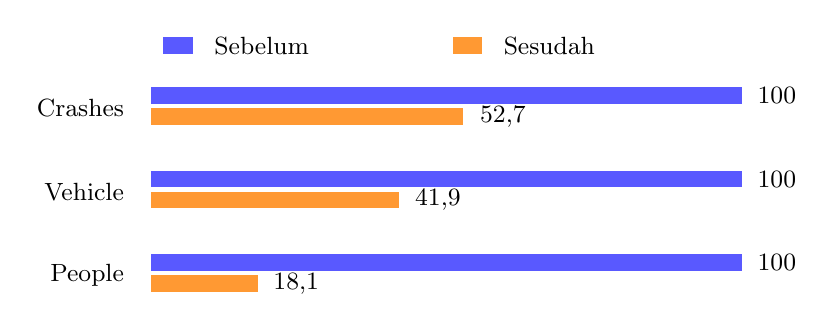
\begin{tikzpicture}[x=0.075cm,y=0.53cm,font=\small]
  \node[anchor=east] at (-3,5.1){Crashes};
  \node[anchor=east] at (-3,3.1){Vehicle};
  \node[anchor=east] at (-3,1.1){People};
  \fill[blue!65] (0,5.2) rectangle (100,5.6);
  \fill[orange!80] (0,4.7) rectangle (52.7,5.1);
  \fill[blue!65] (0,3.2) rectangle (100,3.6);
  \fill[orange!80] (0,2.7) rectangle (41.9,3.1);
  \fill[blue!65] (0,1.2) rectangle (100,1.6);
  \fill[orange!80] (0,0.7) rectangle (18.1,1.1);
  \node[anchor=west] at (101,5.4){100};
  \node[anchor=west] at (54,4.9){52,7};
  \node[anchor=west] at (101,3.4){100};
  \node[anchor=west] at (43,2.9){41,9};
  \node[anchor=west] at (101,1.4){100};
  \node[anchor=west] at (19,0.9){18,1};
  \fill[blue!65] (2,6.4) rectangle (7,6.8);
  \node[anchor=west] at (9,6.6){Sebelum};
  \fill[orange!80] (51,6.4) rectangle (56,6.8);
  \node[anchor=west] at (58,6.6){Sesudah};
\end{tikzpicture}
\caption{Sel kosong pada kolom yang dipertahankan. Nilai sebelum dibuat 100 untuk tiap tabel; batang sesudah menunjukkan sisa persentasenya.}
\end{figure}

Penurunan sel kosong sebagian besar berasal dari label
\texttt{TIDAK\_TERCATAT} dan \texttt{TIDAK\_BERLAKU}; label tersebut
tidak menambah fakta yang sebelumnya hilang. Jumlah kolom berubah dari
49 menjadi 38 setelah seleksi awal dan 67 setelah integrasi pada Crashes;
untuk Vehicle 71 menjadi 17 lalu 38; untuk People 29 menjadi 17 lalu 45.
Kode reduksi akhir memilih 15 kolom dari tabel Crashes terintegrasi.

Pemeriksaan akhir menunjukkan tabel rinci tetap berisi 877.921
kecelakaan, 1.792.372 unit, dan 1.927.657 orang. Sebanyak 871.586
kecelakaan dapat dipetakan ke 77 area; ditambah 6.335 yang belum
terpetakan, jumlahnya tepat 877.921. Jumlah kecelakaan pada 168
kombinasi hari--jam juga 877.921. Koordinat dan cedera yang diperkirakan
mempunyai penanda tersendiri.

\section{Analisis, Temuan Utama, dan Ringkasan}

Jumlah kecelakaan turun dari 117.764 pada 2019 menjadi 92.096 pada 2020
(sekitar 21,8\%), lalu kembali ke kisaran 108--112 ribu per tahun.
Proporsi kecelakaan dengan cedera tercatat naik dari 13,97\% pada 2018
menjadi 16,44\% pada 2025. Ini adalah pola pada data yang dilaporkan,
bukan bukti perubahan risiko perjalanan.

\begin{table}[H]
\centering\small
\caption{Tiga community area dengan jumlah kecelakaan terpetakan tertinggi.}
\begin{tabular}{lrrr}
\toprule
Area & Kecelakaan & Korban & Meninggal\\
\midrule
Austin & 41.495 & 10.695 & 54\\
Near West Side & 40.539 & 8.005 & 34\\
Near North Side & 38.912 & 6.333 & 21\\
\bottomrule
\end{tabular}
\end{table}

Austin memiliki 25,77 korban per 100 kecelakaan, sedangkan Near North Side
16,28. Lima area dengan kecelakaan terbanyak menampung 20,06\% kecelakaan
yang dapat dipetakan. Perbandingan ini belum memperhitungkan jumlah
penduduk, perjalanan, atau kendaraan yang melewati tiap area.

Jumat pukul 15.00 mencatat kecelakaan terbanyak pada tabel hari--jam
(11.630), sedangkan Kamis pukul 17.00 mencatat korban terbanyak
(2.164). Kendaraan jenis \texttt{PASSENGER} tercatat pada 1.087.111 unit
yang terlibat, diikuti SUV sebanyak 254.447 unit. Pada jenis tabrakan,
17,20\% kecelakaan dengan pejalan kaki tergolong berat, dibanding 0,96\%
pada tabrakan belakang. Angka keterlibatan dan persentase ini tidak
menunjukkan penyebab ataupun risiko per perjalanan karena data jumlah
perjalanan tidak tersedia.

\subsection*{Ringkasan}
Seleksi awal mengeluarkan 77 dari 149 kolom sumber tanpa menghapus baris.
Integrasi menghasilkan tiga tabel rinci dan tiga tabel ringkasan. Dari
877.921 kecelakaan, 871.586 dapat dipetakan ke \emph{community area};
6.335 sisanya tetap tercatat tanpa area. Kode reduksi memilih 15 dari 67
kolom tabel kecelakaan terintegrasi untuk analisis umum. Perkiraan tidak
menimpa nilai sumber: 5.909 lokasi dan 891 total cedera masih belum
diketahui. Perbandingan jumlah kecelakaan antarwilayah belum menunjukkan
risiko per perjalanan karena jumlah perjalanan tidak tersedia.

\end{document}
